\documentclass{beamer}
\mode<presentation>
\usetheme{CambridgeUS}
\usepackage[russian]{babel}
\usepackage[utf8]{inputenc}
\usepackage[T2A]{fontenc}
\usepackage{sansmathaccent}

\usepackage{verbatim}
\usepackage{alltt}

\pdfmapfile{+sansmathaccent.map}
\title[Файловая система]{Файловая система в Linux}
\author{Наумов Д.А., доц. каф. КТ}
\date[29.10.2019] {Операционные системы и системное программное обеспечение, 2019}

\begin{document}

%ТИТУЛЬНЫЙ СЛАЙД
\begin{frame}
  \titlepage
\end{frame}
  
%СОДЕРЖАНИЕ ЛЕКЦИИ
\begin{frame}
  \frametitle{Содержание лекции}
  \tableofcontents  
\end{frame}

\section{Обзор файловой системы в Linux}

\begin{frame}{Аксиоматика файловой системы в Linux}
Типичная модель файловой системы Linux:
\begin{itemize}
\item \textbf{нижний уровень}: драйверы устройств и файловых систем, полностью реализован в ядре Linux.
\item \textbf{cредний уровень}: системные вызовы, работающие с файловыми системами и осуществляющие низкоуровневый ввод-вывод, унифицированный интерфейс файловой системы, семь типов файлов: 
\begin{enumerate}
\item каталоги, 
\item символьные устройства, 
\item блочные устройства,
\item обычные файлы, 
\item каналы FIFO, 
\item символические ссылки,
\item сокеты.
\end{enumerate}
\item верхний уровень: библиотеки и приложения, которые создают полноценную иллюзию единого дерева файловой системы.
\end{itemize}
\end{frame}

\begin{frame}[fragile]{Типы файлов. Обычный файл}
\begin{block}{Создадим пустой файл при помощи программы \textit{touch}:}
\begin{alltt}
\$ touch anyfile
\end{alltt}
\end{block}
\begin{block}{Теперь наберем следующую команду:}
\begin{alltt}
\$ ls -l anyfile

-rw-r--r-- 1 nnivanov nnivanov 0 2011-05-06 20:11 anyfile
\end{alltt}
\end{block}
Прочерк в самом начале - поле типа файла с точки зрения среднего уровня реализации
файловой системы. \textit{Если здесь стоит минус, то это обычный файл}.
\end{frame}

\begin{frame}[fragile]{Типы файлов. Каталог}
\begin{block}{Давайте теперь создадим каталог:}
\begin{alltt}
\$ mkdir anydir
\$ ls -l

drwxr-xr-x 2 nnivanov nnivanov 4096 2011-05-06 20:13 anydir/
-rw-r--r-- 1 nnivanov nnivanov 0 2011-05-06 20:11 anyfile
\end{alltt}
\end{block}
В поле типа файла для \textit{anydir} находится символ \textit{d}, показывающий, что это каталог
(\textit{directory}).
\end{frame}

\begin{frame}[fragile]{Типы файлов. Символические ссылки}
Символические ссылки - указатели на другие файлы.
\begin{block}{Создадим символическую ссылку:}
\begin{alltt}
\$ ln -s anyfile anylink
\$ ls -l

drwxr-xr-x 2 nnivanov nnivanov 4096 2011-05-06 20:13 anydir/
-rw-r--r-- 1 nnivanov nnivanov 0 2011-05-06 20:11 anyfile
lrwxrwxrwx 1 nnivanov nnivanov 7 2011-05-06 20:14 anylink -> anyfile
\end{alltt}
\end{block}
Символические ссылки в выводе \textit{ls} обозначаются символом \textit{l} (\textit{link}).
\end{frame}

\begin{frame}[fragile]{Типы файлов. Устройства}
Устройства в Linux могут быть представлены в виде файлов. На среднем уровне
реализации файловой системы под устройствами понимают файлы двух типов:
\begin{itemize}
\item символьные устройства, обозначаемые в выводе программы \textit{ls} символом \textit{c} (character);
\item блочные устройства, обозначаемые символом \textit{b} (\textit{block}).
\end{itemize}
\begin{block}{Введите следующую команду:}
\begin{alltt}
\$ ls -l /dev/null

crw-rw-rw- 1 root root 1, 3 2011-05-06 20:16 /dev/null
\end{alltt}
\end{block}
Вывод программы ls показывает, что /dev/null является символьным устройством.
\end{frame}

\begin{frame}[fragile]{Типы файлов. Устройства}
Унификация обозначения устройств, содержащих файловые системы, жесткие диски, USBнакопители, CD/DVD-приводы, SCSI-устройства:
\begin{block}{Cписок блочных устройств:}
\begin{alltt}
\$ ls -l /dev/sd*

brw-rw---- 1 root disk 8, 0 2011-05-06 18:41 /dev/sda
brw-rw---- 1 root disk 8, 1 2011-05-06 18:41 /dev/sda1
brw-rw---- 1 root disk 8, 2 2011-05-06 18:41 /dev/sda2
brw-rw---- 1 root disk 8, 16 2011-05-06 18:53 /dev/sdb
brw-rw---- 1 root disk 8, 17 2011-05-06 18:53 /dev/sdb1
\end{alltt}
\end{block}
\end{frame}

\begin{frame}[fragile]{Типы файлов. Каналы. Сокеты}
Для взаимодействия процессов существуют особые файлы, которые называются
каналами FIFO (First In First Out) или просто FIFO. 

Эти файлы создаются командой mkfifo и обозначаются в выводе программы ls символом p (pipe):
\begin{block}{Создание канала:}
\begin{alltt}
\$ mkfifo anyfifo
\$ ls -l anyfifo

prw-r--r-- 1 nnivanov nnivanov 0 2011-05-06 20:33 anyfifo
\end{alltt}
\end{block}
\textbf{Сокеты }динамически создаются программами при помощи системного вызова \textit{socket()}. 

Сокеты обозначаются в выводе команды \textit{ls} символом \textit{s} (socket). 
\end{frame}

\begin{frame}[fragile]{Права доступа}
\begin{itemize}
\item Когда процесс пытается получить доступ к какому-нибудь файлу, ядро Linux использует UID текущего процесса для проверки прав доступа.
\item Если проверка не удалась, в ход идет GID (Group ID, идентификатор группы). 
\item Если и здесь доступ закрыт, проверяются права доступа для остальных пользователей.
\end{itemize}
\begin{block}{Права доступа файла shadow}
\begin{alltt}
\$ ls -l shadow

-r--r----- 1 root shadow 1012 2011-03-08 10:03 /etc/shadow
\end{alltt}
\end{block}
Данные о пользователях хранятся в файле /etc/passwd, который открыт для всех, а зашифрованные пароли находятся в
файле /etc/shadow, доступ к которому разрешен только суперпользователю.
\end{frame}

\begin{frame}[fragile]{Права доступа}
Программу su, которая позволяет временно входить в систему на правах другого пользователя. 

\textit{Как su "умудряется" сравнивать введенные вами пароли с содержимым закрытого от посторонних глаз файла /etc/shadow? }
\begin{block}{В первом окне введите команду su:}
\begin{alltt}
\$ su
Password:
\end{alltt}
\end{block}
\begin{block}{Перейдем в другое окно и введем:}
\begin{alltt}
\$ ps -ef
...
nnivanov 17952 9299 0 20:37 pts/1 00:00:00 bash
root 17989 9302 0 20:37 pts/0 00:00:00 su
nnivanov 18008 17952 0 20:37 pts/1 00:00:00 ps -efu
\end{alltt}
\end{block}
\end{frame}

\begin{frame}[fragile]{Права доступа}
\begin{block}{Введите теперь следующую команду:}
\begin{alltt}
\$ ls -l /bin/su

-rwsr-xr-x 1 root root 34500 2010-04-29 19:17 /bin/su
\end{alltt}
\end{block}
\begin{itemize}
\item Триада, показывающая базовые права доступа для пользователя, содержит символ s на месте бита исполнения. 
\item Этот символ означает, что для исполняемого файла установлен бит SUID (Set User IDentifier), который позволяет запускать данную программу от лица владельца ее исполняемого файла. 
\item Существует бит SGID (Set Group IDentifier), который позволяет запускать программу от имени группы, которой принадлежит этот файл.
\end{itemize}
\end{frame}

\begin{frame}[fragile]
К процессу привязано два идентификатора пользователя:
\begin{itemize}
\item реальный UID (Real UID, RUID или просто UID);
\item эффективный UID (Effective UID или просто EUID).
\end{itemize}
В большинстве случаев эти идентификаторы равны. Но если для исполняемого
файла программы установлен бит SUID, то ситуация меняется. 
\begin{block}{Пример}
когда пользователь anyuser запускает программу su, то реальный UID процесса равен идентификатору пользователя anyuser, а эффективный UID равен идентификатору пользователя root.
\end{block}
\begin{block}{Установить бит SUID для исполняемого файла:}
\begin{alltt}
\$ chmod u+s file
\end{alltt}
\end{block}
\begin{block}{Установить бит SGID для исполняемого файла:}
\begin{alltt}
\$ chmod g+s file
\end{alltt}
\end{block}
\end{frame}

\begin{frame}[fragile]
Расширенные права доступа позволяют задействовать еще один бит, который называется битом SVTX или липким битом (sticky). В каталоге с установленным битом SVTX каждый может создавать, удалять и переименовывать файлы, не мешая другим пользователям делать то же самое.  
\begin{block}{Каталог /tmp, доступен всем для хранения временных файлов:}
\begin{alltt}
\$ ls -l / | grep tmp

drwxrwxrwt 63 root root 12288 2011-05-06 20:42 tmp/
\end{alltt}
\end{block}
\begin{block}{Назначить каталогу directory липкий бит:}
\begin{alltt}
\$ chmod +t directory
\end{alltt}
\end{block}
\end{frame}

\begin{frame}[fragile]{Служебные файловые системы}
\begin{block}{Файловая система /dev}
\begin{itemize}
\item хранилище файлов символьных и блочных устройств.
\end{itemize}
\end{block}
\begin{block}{Файловая система /proc}
\begin{itemize}
\item  была создана для предоставления пользователю информации о работающих процессах; 
\item  затем туда стали помещать туда <<полезную>> информацию (версия ОС, объем оперативной памяти, сообщения ядра и т. п.);
\item  в некоторые файлы дерева /proc можно писать, обеспечивая тем самым динамическое конфигурирование ядра.
\end{itemize}
\end{block}
\begin{block}{Файловая система /tmp}
\begin{itemize}
\item предназначена для хранения временных файлов. 
\item может располагаться как на диске, так и в памяти.
\end{itemize}
\end{block}
\end{frame}

\begin{frame}[fragile]{Устройства}
На среднем уровне реализации файловой системы все устройства представляются двумя типами файлов:
\begin{block}{Символьные устройства (character devices)}
\begin{itemize}
\item особенность - механизм последовательного ввода-вывода;
\item рассматриваются не в виде линейного массива данных, а как поток информации.
\end{itemize}
\end{block}
\begin{block}{Блочные устройства (block devices)}
\begin{itemize}
\item читают и записывают данные блоками фиксированного размера с использованием механизма буферизации. 
\item файлы устройств этого типа чаще всего применяются для дисковых накопителей и для дисковых разделов. 
\item некоторые сетевые устройства также могут быть представлены файлами этого типа.
\end{itemize}
\end{block}
\end{frame}

\begin{frame}[fragile]
\begin{block}{Файлы устройств обычно создаются в Linux программой mknod}
\begin{alltt}
\$ mknod [-m MODE] NAME TYPE MAJOR MINOR
\end{alltt}
\end{block}
\begin{itemize}
\item -m принимает независимый аргумент MODE, который является правами доступа создаваемого файла в восьмеричном представлении.
\item NAME - имя файла устройства.
\item TYPE может быть представлен одним из следующих символов: c, b, u или p. 
\begin{itemize}
\item c - будет создано символьное устройство. 
\item b - инициирует создание блочного устройства. 
\item u - блочное устройство, но с выключенным механизмом буферизации (unbuffered). 
\item p - создание именованного канала FIFO.
\end{itemize}
\item MAJOR — это старший номер устройства (номер драйвера).
\item MINOR — младший номер устройства (форма применения драйвера).
\end{itemize}
см. Documentation/devices.txt
\end{frame}

\begin{frame}[fragile]
\begin{block}{Монтирование файловых систем}
позволяет объединять различные файловые системы в одно дерево.
\end{block}
\begin{alltt}
\$ mount
/dev/sda2 on / type ext4 (rw)
none on /proc type proc (rw)
none on /proc/sys/fs/binfmt_misc type binfmt_misc (rw)
/dev/sdb1 on /media/4779-86EA type vfat
(rw,nosuid,nodev,uhelper=udisks,uid=500,gid=500,
shortname=mixed,dmask=0077, utf8=1,flush)
\end{alltt}
DEVICE on MOUNTPOINT type FSTYPE (FLAGS)
\begin{itemize}
\item DEVICE — имя устройства.
\item MOUNTPOINT — точка монтирования: каталог, являющийся как бы <<порталом>> для смонтированной файловой системы. 
\item FSTYPE — тип файловой системы с точки зрения нижнего уровня ее реализации.
\item FLAGS — опции монтирования. 
\end{itemize}
\end{frame}

\section{Чтение информации о файловой системе}

\begin{frame}[fragile]{Семейство statvfs()}
\begin{block}{Информация о смонтированных файловых системах обычно хранится в файле/etc/mtab:}
\begin{alltt}
\$ cat /etc/mtab
/dev/sda2 / ext4 rw 0 0
none /proc proc rw 0 0
none /proc/sys/fs/binfmt_misc binfmt_misc rw 0 0
\end{alltt}
\end{block}
Каждая строка /etc/mtab соответствует одной смонтированной файловой системе и содержит шесть полей:
\begin{itemize}
\item Первое поле - носитель файловой системы.
\item Второе поле - точка монтирования.
\item Третье поле - тип файловой системы.
\item Четвертое поле - флаги монтирования.
\item Пятое поле используется утилитой суперпользователя dump.
\item Шестое поле необходимо для утилиты fsck.
\end{itemize}
\end{frame}

\begin{frame}[fragile]
\begin{block}{Функции для разбора файла /etc/mtab:}
\begin{alltt}
FILE * setmntent (const char * FILENAME, const char * MODE);
struct mntent * getmntent (FILE * FILEP);
int endmntent (FILE * FILEP);
\end{alltt}
\end{block}
\begin{itemize}
\item setmntent() открывает файл, в котором содержится список смонтированных файловых систем;
\item getmntent() извлекает следующую запись о файловой системе. 
\item endmntent() вызывается по окончании чтения записей о файловых системах.
\end{itemize}
Поля структуры mntent соответствуют полям /etc/mtab:
\begin{alltt}
  char *mnt_fsname;
  char *mnt_dir;
  char *mnt_type;
  char *mnt_opts;
  int mnt_freq;
  int mnt_passno;
\end{alltt}
\end{frame}

\begin{frame}[fragile]
Более подробную информацию о файловых системах позволяют получить следующие функции, объявленные в заголовочном файле sys/statvfs.h:
\begin{alltt}
int statvfs (const char * PATH, struct statvfs * FS);
int fstatvfs (int FD, struct statvfs * FS);
\end{alltt}
\begin{itemize}
\item \textit{f\_bsize} - целое число, содержащее размер блока файловой системы в байтах.
\item \textit{f\_blocks} - целое число, показывающее количество блоков в файловой системе.
\item \textit{f\_bfree} - целое число, содержащее количество свободных блоков в файловой системе.
\item \textit{f\_bavail} содержит число доступных блоков, без учета резервных блоков, которые некоторые файловые системы выделяют для специального использования.
\item \textit{f\_namemax} - целое число, показывающее максимально возможную длину имени файла в данной файловой системе. \end{itemize}
\end{frame}

%\section{Чтение каталогов}
%\section{Операции над файлами}

%\begin{figure}[h]
%\centering
%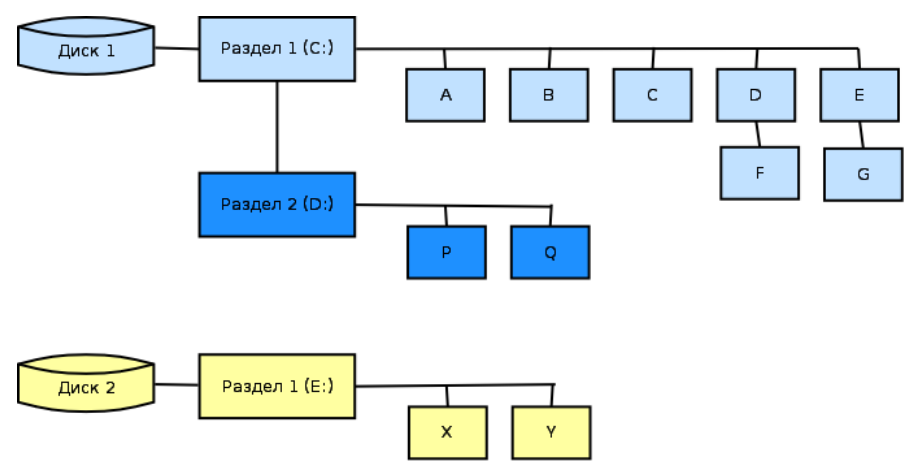
\includegraphics[scale=0.5]{images/lec09-pic01.png}
%\end{figure}

\end{document}